% Source: methodology-zh-v3.md, section V
% Chinese text retained; Drive comment metadata is kept only in the local backup.
\section{评估}\label{sec:evaluation}

\subsection{实验设置}\label{sec:evaluation-a}

我们采用``Thor 实测校准 VLM 访存模型 + Ramulator2 周期精确仿真 PIM''的评估方法。GPU 侧，在 NVIDIA Thor 上用 OpenPI 的 PyTorch 实现实测 \(\pi_{0.5}\)（MHA8 配置，BF16，batch=1，动作块长度 H=16，10 个去噪步，3 路相机加 200 个文本 token），得到 VLM 各 kernel 的时长与读写字节，以及 AE 非线性算子的时长。PIM 侧，基于 Ramulator2 构建周期精确仿真器，在同一个内存控制器中同时模拟 VLM 访存与 PIM 命令；DRAM 时序取自 JEDEC JESD209-5C 的 LPDDR5X-8533 速档{[}待引用{]}。

面积评估方面，VLA-PIM相比LPDDR5X，每个 PIM bank 新增 1 KiB Input Buffer、2 KiB Output Buffer、MAC 单元与 RoPE 单元，以及 Row Buffer \(\rightarrow\) Input Buffer 的广播通路。我们沿用 AttAcc 的方法估计面积：先在逻辑工艺下综合新增单元，再按 DRAM 工艺相对逻辑工艺的面积代价折算到 DRAM 裸片上【待核：AttAcc 原文采用的工艺节点、折算系数及其引用来源】。【待补-M11：面积数值】

% Source caption: 表 VII：主要仿真参数
\begin{table}[t]
\centering
\caption{主要仿真参数}
\label{tab:sim-params}
\small
\begin{tabularx}{\linewidth}{@{}>{\raggedright\arraybackslash}p{0.26\linewidth} >{\raggedright\arraybackslash}X@{}}
\toprule
参数 & 取值 \\
\midrule
内存 & LPDDR5X-8533，16 通道 \(\times\) x16，每通道 2 rank，BG 模式 4 BG \(\times\) 4 bank \\
时钟 & CK = 0.938 ns，WCK:CK = 4:1，WCK always-on \\
主要时序 (CK) & CL/CWL 23/12；tRCD 20(读)/9(写)；tRP 20(pb)/23(ab)；tRAS/tRC 45/65；tRRD/tFAW 4/16；tWTR\_\allowbreak{}S/L 7/13；tWR 37；tCCD\_\allowbreak{}L 4 \\
刷新 (CK) & tRFCab/pb 224/128；tREFI/tREFIpb 4164/520 \\
\bottomrule
\end{tabularx}
\end{table}


\subsection{总体性能}\label{sec:evaluation-b}

VLA-PIM 的目标是提高 AE 的推理频率。若每次 AE 推理都使用最新的 VLM KV cache，第 n 帧的 AE 就必须等待第 n 帧的 VLM 完成，因此相邻两次 AE 的间隔为

\begin{equation}
t_{\mathrm{AE\text{-}AE}} = t_{\mathrm{AE,solo}} + t_{\mathrm{VLM,solo}} - t_{\mathrm{overlap}}.
\label{eq:ae-interval}
\end{equation}

其中 \(t_{\mathrm{overlap}}\) 是 VLM 与（上一帧）AE 真正重叠执行的时间。串行执行时 \(t_{\mathrm{overlap}}\) = 0；\(t_{\mathrm{overlap}}\) 越大，AE 的推理频率 1/\(t_{\mathrm{AE\text{-}AE}}\) 越高。表~\ref{tab:performance} 给出各配置的结果。仿真配置的 \(t_{\mathrm{AE,solo}}\) 与 \(t_{\mathrm{VLM,solo}}\) 均取同一设计单独运行的仿真结果（\(t_{\mathrm{VLM,solo}}\) = 65.94 ms）。

% Existing data retained; English captions and references synchronized with the 2026-11-17 source.
\begin{table*}[!t]
\caption{Asynchronous VLA Inference Cycle and AE Output Rate}
\label{tab:performance}
\centering
\footnotesize
\setlength{\tabcolsep}{2.6pt}
\begin{tabular*}{\textwidth}{@{\extracolsep{\fill}}lrrrrrr@{}}
\toprule
\textbf{Config} & \hcell{\textbf{AE done}\\(ms)} & \hcell{\textbf{VLM prog.}\\(ms)} & \hcell{$\bm{t_{\mathrm{overlap}}}$\\(ms)} & \hcell{$\bm{T_{\mathrm{async\_VLA}}}$\\(ms)} & \hcell{\textbf{Rate}\\(Hz)} & \hcell{\textbf{vs.}\\\textbf{a-serial}} \\
\midrule
a-serial (Thor) & 73.98 & --- & 0 & 141.29 & 7.08 & 1.00$\times$ \\
a-dual (Thor) & --- & --- & 4.31 & 137.07 & 7.30 & 1.03$\times$ \\
b & 56.95 & 0 & 0 & 122.88 & 8.14 & 1.15$\times$ \\
c & 60.33 & 47.48 & 36.12 & 86.77 & 11.53 & 1.63$\times$ \\
d & 57.90 & 47.42 & 36.33 & 84.04 & 11.90 & 1.68$\times$ \\
e & 56.83 & 47.16 & 36.35 & 83.57 & 11.97 & 1.69$\times$ \\
f & 69.27 & 60.15 & 54.80 & 78.17 & 12.79 & 1.81$\times$ \\
\textbf{g (\sys{})} & 68.64 & 60.30 & 54.96 & \textbf{77.68} & \textbf{12.87} & \textbf{1.82}$\bm{\times}$ \\
\bottomrule
\end{tabular*}
\par\smallskip
\parbox{\textwidth}{\scriptsize ``VLM prog.'' is the VLM progress completed before the AE finishes.}
\end{table*}


主要观察如下：

\begin{enumerate}
\def\labelenumi{\arabic{enumi}.}

\item
  \textbf{异构本身的收益。} 把 AE 的线性层搬到 PIM 后，即使串行执行（b），\(t_{\mathrm{AE\text{-}AE}}\) 也比 a-serial 缩短到 1/1.15：AE 完成时间为 56.95 ms，而 Thor 上 compile 后的 AE 实测为 73.98 ms；其中 PIM 部分 46.01 ms，占 AE 时间的 80.8\%。
\item
  \textbf{rank 划分带来的并发收益。} 让 VLM 与 AE 并发（c），\(t_{\mathrm{overlap}}\) 达到 36.12 ms，\(t_{\mathrm{AE\text{-}AE}}\) 从 122.88 ms 降到 86.77 ms（1.42\(\times\)）。AE 本身只慢了 3.38 ms（5.9\%），其中 PIM 阶段因 GPU 并发只被拉长 0.51 ms，说明 rank 划分确实为两者提供了相对独立的资源。
\item
  \textbf{布局与 RoPE。} 在流式数据流下，token-wise 布局（d）比 feature-wise（c）快 2.73 ms（3.1\%），片内 RoPE（e）再快 0.47 ms。收益主要来自 AE 侧：DQ 流量减少，GPU 非线性工作从 10.93 ms 降到 8.11 ms。
\item
  \textbf{输入预装载。} 预装载（g）让 AE 的 PIM 部分变长，AE 完成时间增加 11.8 ms；但 AE 结束时 VLM 已完成 60.30 ms 的工作（流式只有 47.16 ms，+27.8\%），\(t_{\mathrm{overlap}}\) 从 36.35 ms 增加到 54.96 ms（+51.2\%）；1416 个 VLM kernel 中完成了 1366 个（流式为 1271 个），剩余的 VLM 尾部从 26.74 ms 缩短到 9.03 ms。最终 \(t_{\mathrm{AE\text{-}AE}}\) 从 83.57 ms 降到 77.68 ms（-7.0\%），AE 推理频率达到 a-serial 的 1.82\(\times\)、a-dual 的 1.76\(\times\)。
\end{enumerate}

\begin{figure*}[!t]
\centering
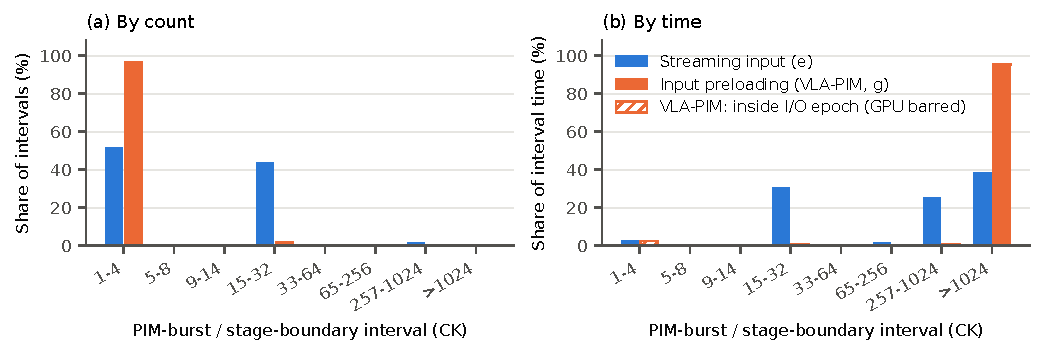
\includegraphics[width=\textwidth]{figures/fig_dq_gap_distribution.pdf}
\setcounter{figure}{7}
\caption{PIM 相邻数据突发间隔的分布（物理通道 0，完整 18 \(\times\) 10 调度）。(a) 按数量；(b) 按时间，斜线部分为位于 I/O epoch 内的间隔。虚线左侧（\textless{} 15 CK）的间隔无法插入一次 GPU 读。}\label{fig:dq-gaps}
\end{figure*}


\textbf{GPU 在 PIM 计算期间获得的带宽。} 我们统计所有 PIM 阶段内（16 通道合计）GPU 获得的 DQ 带宽。VLM 单独运行时，GPU 平均获得 221.6 GB/s。流式供数下，PIM 阶段内 GPU 只能获得 173--175 GB/s，保持率为 78.2\%--78.9\%；预装载后提高到 204.2 GB/s，保持率为 92.2\%。同时，PIM 阶段内 GPU 搬运的数据从 7.53 GiB 增加到 11.35 GiB（+50.7\%）。这说明预装载把原本碎片化、GPU 无法利用的 DQ 空隙合并成了 GPU 可以连续使用的窗口。

\textbf{DQ 空隙分布。} 图~\ref{fig:dq-gaps} 统计了完整 18 层 \(\times\) 10 步调度中，物理通道 0 上 PIM 相邻数据突发之间的间隔。流式供数（e）下共有 126 万个间隔，其中 52.9\% 短于 15 CK，按 DQ 时序无法插入任何一次 GPU 读；按时间计，只有 38.8\% 的间隔时间落在长于 1024 CK 的窗口中。预装载（g）后，间隔数减少到 77 万个（-38.7\%）。虽然按数量计 97.2\% 的间隔短于 15 CK，但它们都是 I/O epoch 内连续传输之间的间隔，而 GPU 在 epoch 内本就不发请求；在 epoch 之外，99.8\% 的间隔时间落在长于 1024 CK 的窗口中。需要说明的是，这些间隔中可能已经包含 GPU 的传输，因此``无法插入 GPU 读''只是基于 DQ 时序的几何判断，并非实测的 GPU 不可用时间。


\textbf{C/A 占用。} 在 PIM 阶段内，PIM rank 占用的外部 C/A 周期比例为：c 14.2\%、d 16.2\%、e 16.2\%、f 14.4\%、g 14.4\%。g 中加上 GPU 的 C/A 占用（40.0\%），C/A 总占用为 54.4\%，C/A 总线仍有余量。预装载在为 GPU 释放 DQ 的同时，并未增加 C/A 负担。

\subsection{讨论：VLM 与 AE 的解耦}\label{sec:evaluation-c}

\begin{figure}[!t]
\centering
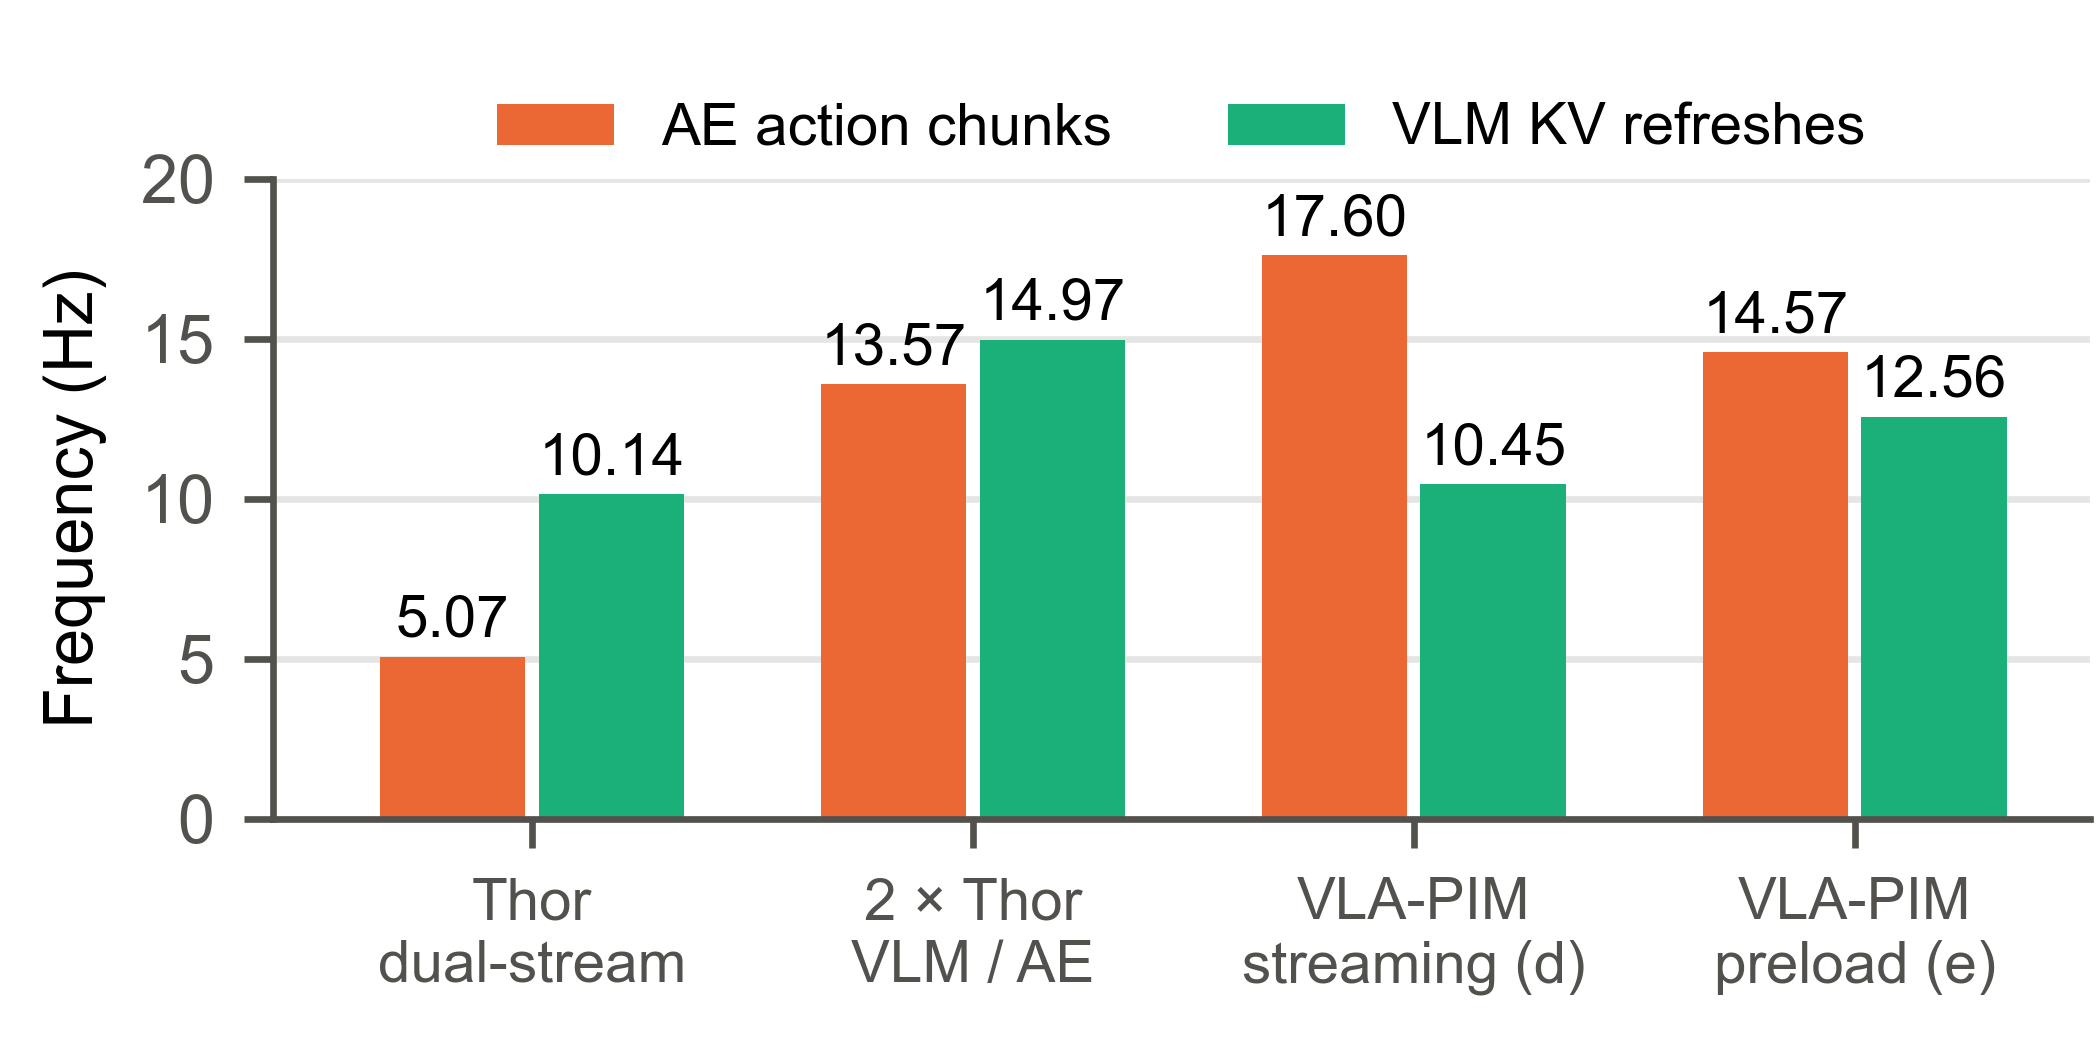
\includegraphics[width=\columnwidth]{figures/fig8_decoupled_rate.png}
\caption{AE action-chunk rate and VLM KV refresh rate under decoupled execution.
Thor dual-stream: VLM and AE sharing one GPU;
2$\times$ Thor: dedicated GPUs for VLM and AE.}
\label{fig:decoupled-rates}
\end{figure}


VLA-PIM 的异构结构天然支持 VLM 与 AE 解耦。配合合适的异步算法，VLM 可以较慢地更新 KV cache，PIM 则以更高的频率执行 AE 推理，实现真正的异步执行。单 GPU 上则很难做到：Thor 双 stream 连续运行时，AE 只有 5.13 Hz，VLM 刷新频率为 10.13 Hz。增加 GPU 算力也无法缓解 AE 的访存受限：即使让 AE 独占 Thor GPU，其频率也只有 13.57 Hz。在 VLA-PIM 中，AE 与 VLM 解耦运行时，AE 频率约为 14.57 Hz，是 Thor 双流的 2.84\(\times\)，并超过 AE 独占 GPU 的频率；同时 VLM 刷新频率约为 12.56 Hz，只比 VLM 独占 GPU（14.97 Hz）低 16.1\%，比 Thor 双流高 24.0\%（图~\ref{fig:decoupled-rates}）。也就是说，VLA-PIM 只让 GPU 上 VLM 的更新频率下降约 1/6，就使 AE 推理频率达到双流 GPU 基线的近 3 倍。这里的频率由单个重叠窗口外推得到：AE 频率取 1/AE 完成时间，VLM 频率按窗口内完成的 VLM 工作量折算，尚未做多帧连续仿真。
